\subsection{Par\'ametros estructurales del $\mathbf{YCrO_{3}}$ con arreglos 
antiferromagn\'eticos tipo A, C y G}

En la tabla \ref{tabla_YCrO3_parametro_red} se recogen los par\'ametros 
estructurales (a,b,c) del $YCrO_{3}$ perteneciente al espacio de grupo Pnma, 
para los tres arreglos antiferromagn\'eticos.Los par\'ametros se obtuvieron de 
la relajaci\'on de la estructura cristalina los par\'ametros son muy cercanos a 
valores experimentales obtenidos con difracci\'on de rayos X 
\cite{remeika1956,ramesha2007}

% ------------------------------
% TABLA: parametros optimizados
% ------------------------------

\begin{table}[H]
	\begin{center}
		\begin{tabular}{cccc}
			\hline
			    & \textbf{a (\AA)} & \textbf{b (\AA)} & \textbf{c 
			(\AA)} \\
			\hline \hline
			AF-A & $5.14$ & $5.49$ & $7.41$ \\
			\hline
			AF-C & $5.15$ & $5.47$ & $7.42$ \\
			\hline
			AF-G & $5.14$ & $5.47$ & $7.41$ \\
			\hline
			\cite{remeika1956} & $5.238$ & $5.518$ & $7.54$ \\
			\hline
			\cite{ramesha2007} & $5.515$ & $5.234$ & $7.521$ \\
			\hline
		\end{tabular}
		\singlespace
		\caption[Par\'ametros de red optimizados del $YCrO_{3}$]{Comparaci\'on 
			de los par\'ametros estructurales de los tres arreglos 
			antiferromagn\'eticos, con valores obtenidos de difracci\'on de 
			rayos X.}
		\label{tabla_YCrO3_parametro_red}
	\end{center}
\end{table}

\noindent Se hall\'o que el arreglo tipo G posee el volumen m\'as peque\~no lo 
cual se 
corresponde con la energ\'ia total m\'as baja, lo cual lo hace el 
m\'as estable, 
como se muestra en la tabla \ref{tabla_YCrO3_ener_vol_mag}.

% ------------------------------------------------------------------------
% TABLA: energia total, volumen de la celda, momento magnetico del hierro
% ------------------------------------------------------------------------

 \begin{table}[H]
	\begin{center}
		\begin{tabular}{cccc}
			\hline
			\textbf{Tipo} & \textbf{Energ\'ia total (eV)} & \textbf{Volumen 
			(\AA $^{3}$)} & \textbf{Momento magn\'etico Cr ($\mu _{B}$)}\\
			\hline \hline
			AF-A & $-1462.919$ & $209.09$ & $2.75$ \\
			\hline
			AF-C & $-1462.923$ & $209.03$ & $2.70$ \\
			\hline
			AF-G & $-1462.926$ & $208.59$ & $2.65$ \\
			\hline
		\end{tabular}
		\singlespace
		\caption{Energ\'ia total, volumen de la celda y momento magn\'etico del 
		\'atomo de cromo,
			para los tres arreglos antiferromagn\'eticos}
		\label{tabla_YCrO3_ener_vol_mag}
	\end{center}
\end{table}

\noindent Los momentos magn\'eticos del cromo de los tres arreglos 
antiferromagn\'eticos 
mostrados en la tabla \ref{tabla_YCrO3_ener_vol_mag} se encuentran pr\'oximos 
al valor de 3 $\mu _{B}$, un comportamiento esperado \cite{nair2013,serrao2005}.


\subsection{Estructura de bandas de energ\'ia del $\mathbf{YCrO_{3}}$ con      
    arreglo antiferromagn\'etico tipo A}

% ----------------------------
% FIGURA: banda YCrO3 tipo A
% ----------------------------

\begin{figure}[H]
	\centering
	\includegraphics[width=0.7\textwidth]{contenido/resultados/cromita_itrio/img_cromita_itrio/YCrO3_bandas_A_inf.png}
	\singlespace
	\caption[Bandas de energ\'ia del $YCrO_{3}$ con arreglo 
	antiferromagn\'etico tipo A]{Estructura de bandas de energ\'ia del 
	$YCrO_{3}$ con arreglo antiferromagn\'etico tipo A. La linea roja marca el 
	nivel de fermi. Los puntos de alta simetr\'ia tomados en la primera zona de 
	brillouin son $\Gamma - X - S - Y - \Gamma$.}
	\label{yco_band_a}
\end{figure}


La figura \ref{yco_band_a} muestra la estructura de bandas de energ\'ia del 
$YCrO_{3}$ con arreglo antiferromagn\'etico tipo A. Las energ\'ias 
fueron escaladas 
respecto al nivel de fermi, que es tomado como el cero de la escala 
vertical. Se observa un gap de 
energ\'ia de $1.3$ eV. El 
gap se halla entre el m\'aximo de la banda de valencia y el m\'inimo de la 
banda de conducci\'on; estando ambos ubicados en el punto de alta simetr\'ia 
$\Gamma$. Por debajo del nivel de fermi en la banda de valencia 
alrededor del nivel de energ\'ia de -3 eV se observa una franja que no 
posee bandas de energ\'ia. 

\subsection{Densidad de estados del $\mathbf{YCrO_{3}}$ con arreglo      
    antiferromagn\'etico tipo A}

% -------------------------------------------
% FIGURA: densidades de estado YCrO3 tipo A
% -------------------------------------------

\begin{figure}
    \centering
    \subfloat[]{
        \label{yco_tot_a}
        \includegraphics[width=0.5\textwidth]{contenido/resultados/cromita_itrio/img_cromita_itrio/YCrO3_DOS_A_inf.png}}
    \subfloat[]{
        \label{yco_y_a}
        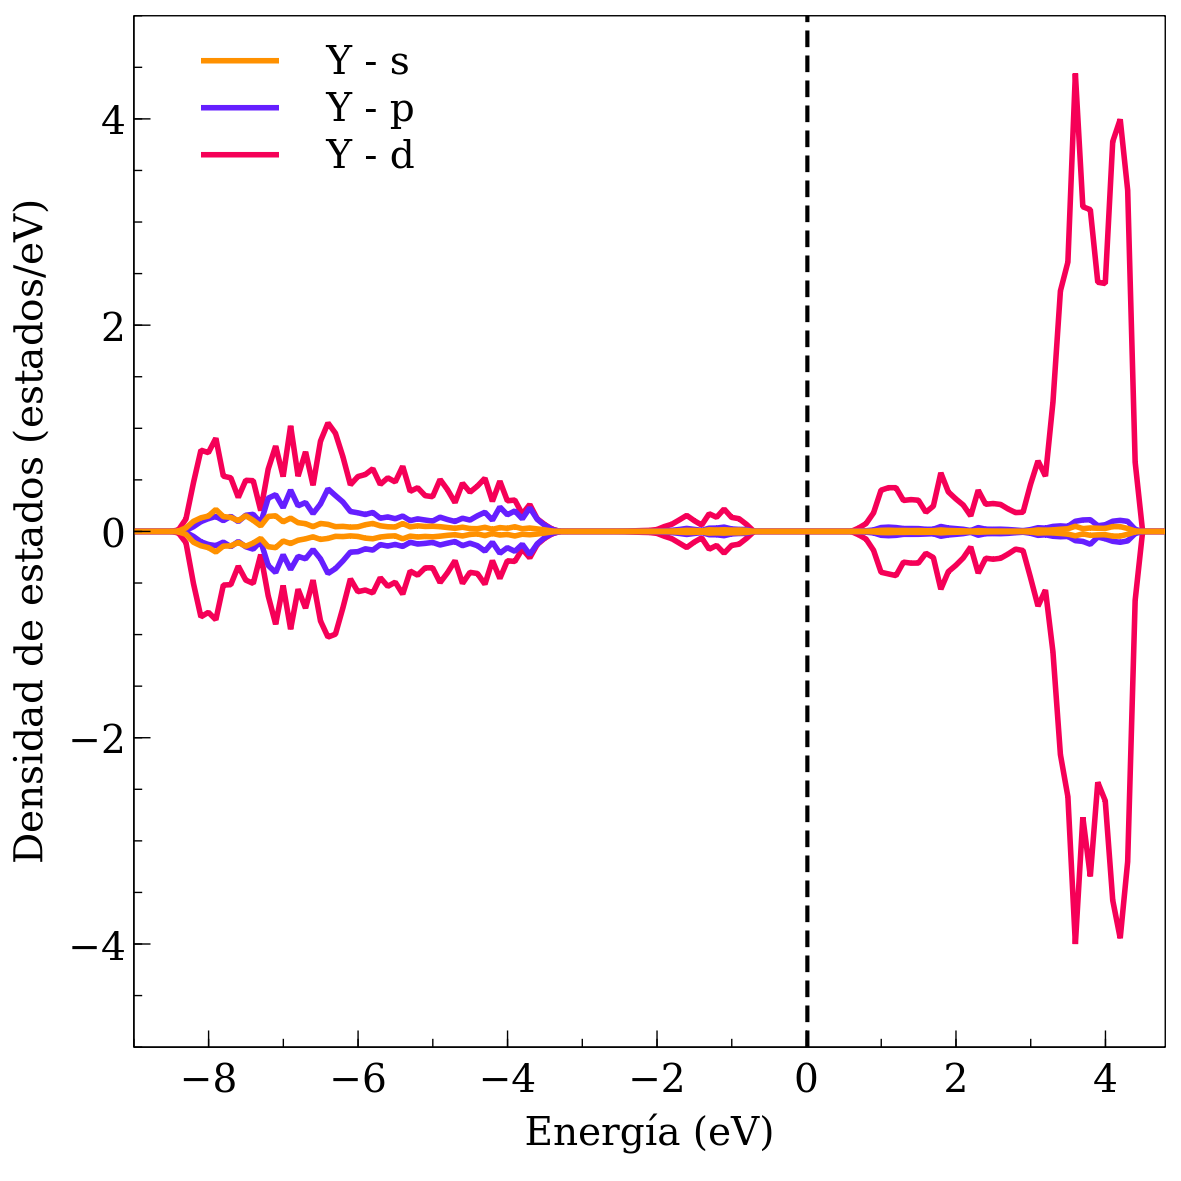
\includegraphics[width=0.5\textwidth]{contenido/resultados/cromita_itrio/img_cromita_itrio/YCrO3_DOS_Y_A_inf.png}}
    
    \subfloat[]{
        \label{yco_cr_a}
        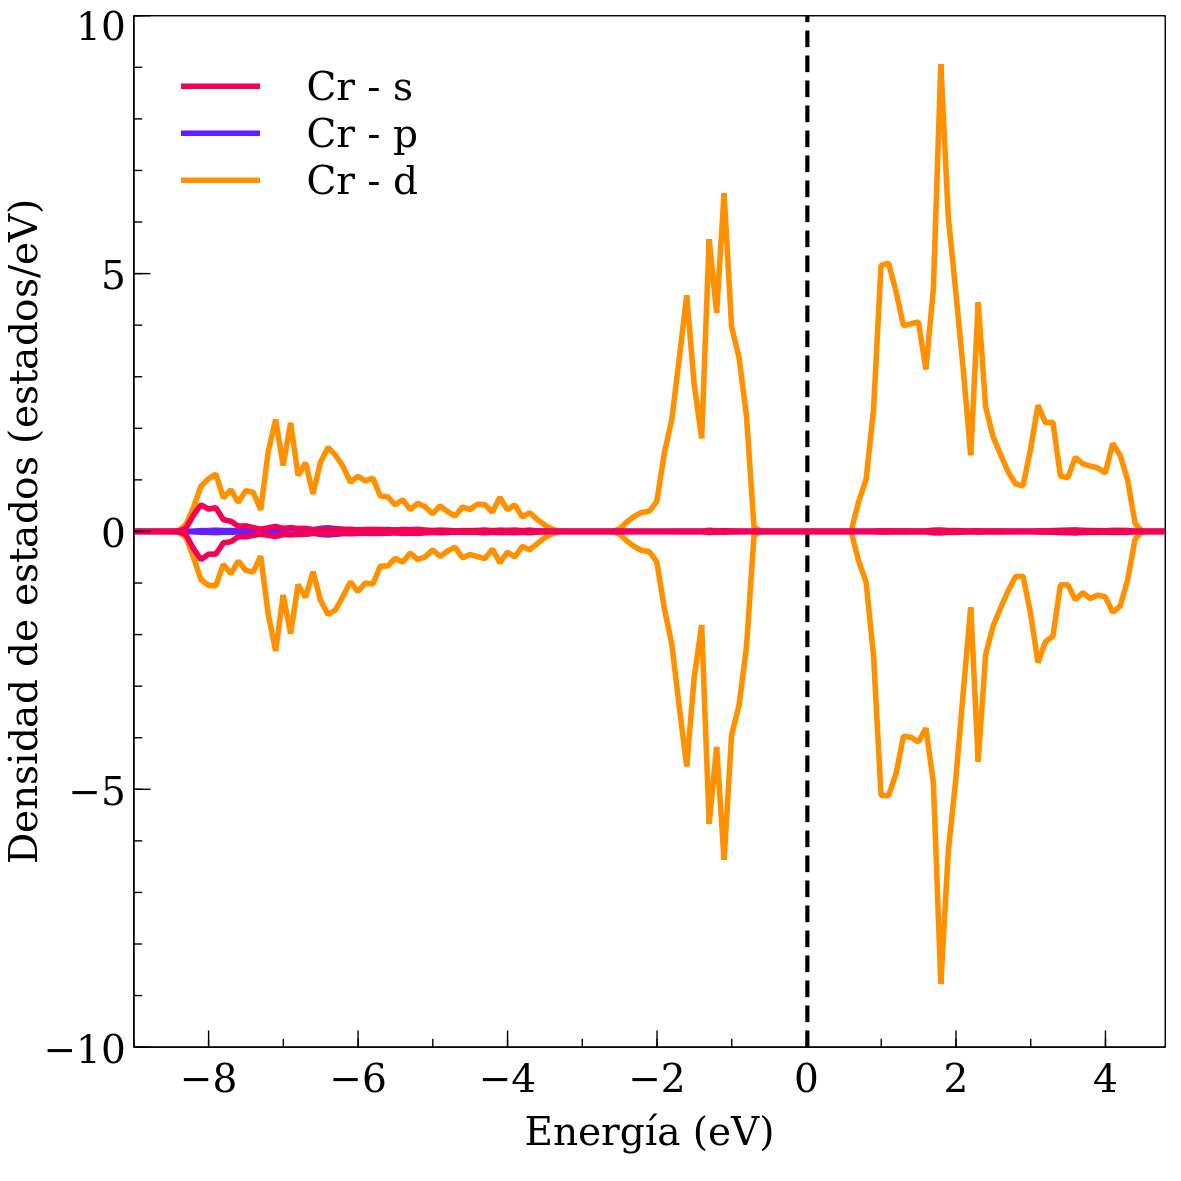
\includegraphics[width=0.5\textwidth]{contenido/resultados/cromita_itrio/img_cromita_itrio/YCrO3_DOS_Cr_A_inf.png}}
    \subfloat[]{
        \label{yco_o_a}
        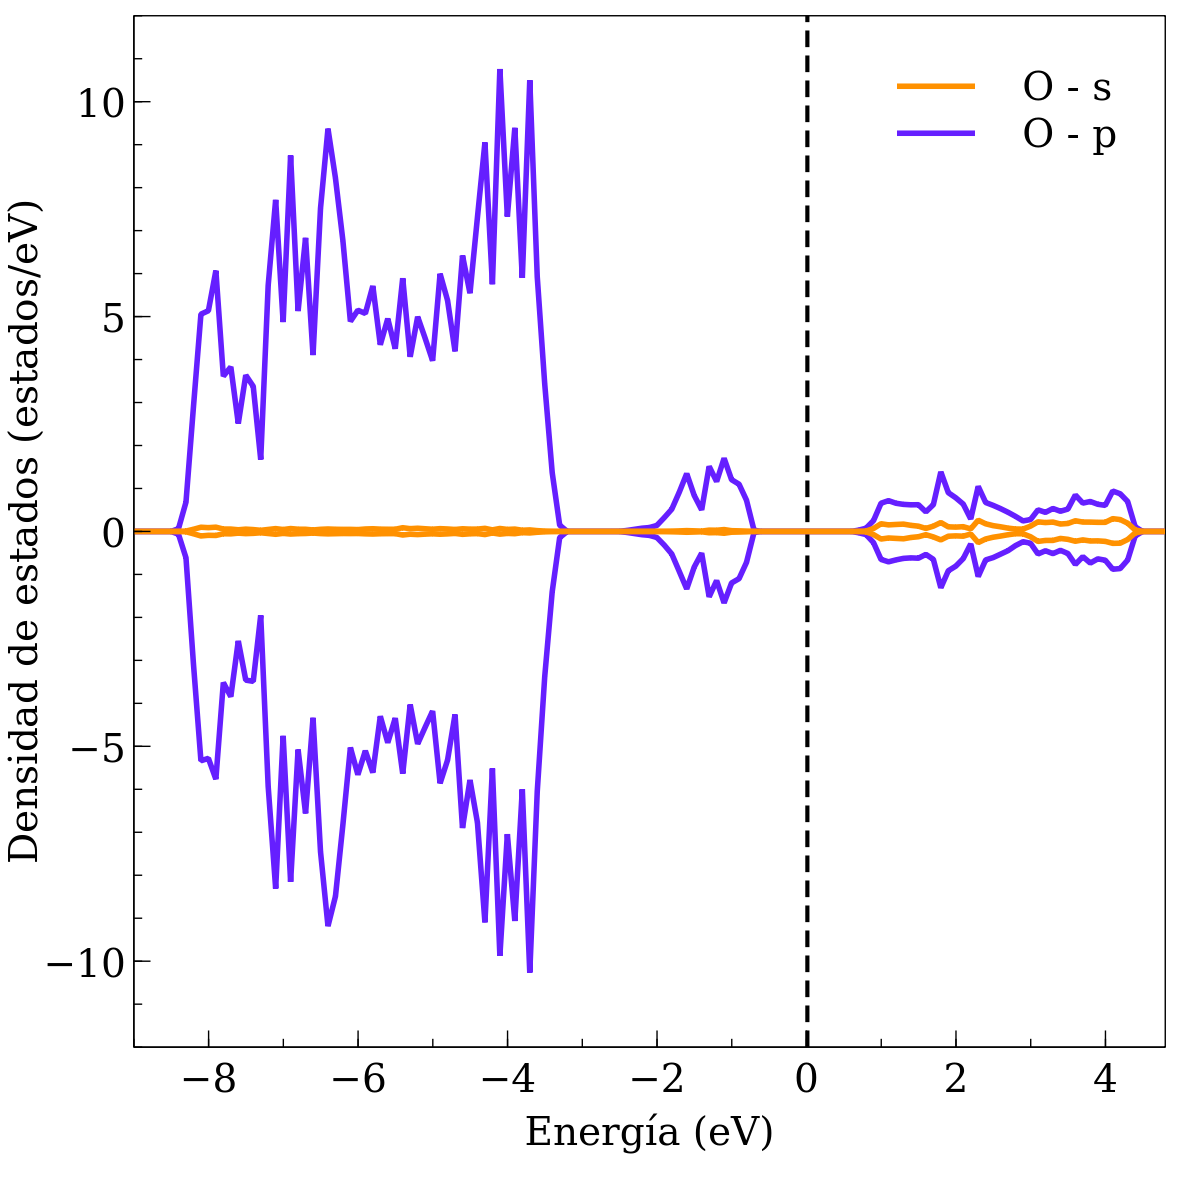
\includegraphics[width=0.5\textwidth]{contenido/resultados/cromita_itrio/img_cromita_itrio/YCrO3_DOS_O_A_inf.png}}
    \singlespace
    \caption[Densidad de estados del $YCrO_{3}$ con arreglo 
    antiferromagn\'etico tipo A]{Densidad de estados del $YCrO_{3}$ 
    con arreglo 
        antiferromagn\'etico tipo A. La linea negra en cero indica el 
        nivel de 
        fermi. \ref{yco_dos_a} \subref{yco_tot_a} Densidad de estados total y 
        de cada elemento. \ref{yco_dos_a} \subref{yco_y_a} 
        Densidad de 
        estados para los orbitales s, p, d del itrio. \ref{yco_dos_a} 
        \subref{yco_cr_a} Densidad de 
        estados para 
        los orbitales s, p ,d del Cromo. \ref{yco_dos_a} \subref{yco_o_a} 
        Densidad de estados para 
        los orbitales 
        s, p del Oxigeno.}
    \label{yco_dos_a}
\end{figure}

La figura \ref{yco_dos_a} \subref{yco_tot_a} muestra la densidad de estados 
total para 
cada 
elemento que compone el $YCrO_{3}$.Las energ\'ias fueron escaladas 
respecto al 
nivel de fermi que se tomo como cero de la escala horizontal, y la 
escala 
vertical positiva y negativa corresponden a los espines up y down 
respectivamente. En la banda de conducci\'on cerca del nivel de fermi 
hasta el nivel de energ\'ia de 3 eV los estados de cromo poseen la 
mayor densidad que oscila entre 5 estados/eV y 10 estados/eV, seguido 
por la densidad de estados del ox\'igeno que es aproximadamente 2 
estados/eV y en este intervalo de energ\'ia la densidad de estados de 
itrio es muy baja. Aproximadamente a partir de los 3 eV la densidad de 
estados de itrio aumenta, alcanzando aproximadamente 4 estados/eV, 
seguido por la densidad de estados de cromo y ox\'igeno que son 
similares entre s\'i. En la banda de valencia cerca del nivel de fermi 
hasta aproximadamente -2 eV la densidad de estados de cromo es la 
mayor con aproximadamente 7 estados/eV, seguida por la densidad de 
estados de ox\'igeno con 2 estados/eV y la densidad de estados de 
itrio en este intervalo de energ\'ia es casi nula. A partir de -4 eV 
hasta -8 eV la densidad de estados de ox\'igeno es la mayor con un 
m\'aximo de 9 estados/eV, seguida por la densidad de estados de itrio 
y cromo que son similares entre s\'i con un valor de 2 estados/eV.


\noindent La figura \ref{yco_dos_a} \subref{yco_y_a} muestra la densidad de 
estados parcial del 
itrio para 
cada 
uno de los orbitales \textbf{s}, \textbf{p} y \textbf{d}.Las 
energ\'ias fueron escaladas 
respecto al 
nivel de fermi que se tomo como cero de la escala horizontal, y la 
escala 
vertical positiva y negativa corresponden a los espines up y down 
respectivamente. En la banda de conducci\'on cerca del nivel de fermi 
hasta aproximadamente 3 eV la densidad del orbital \textbf{d} es la 
mayor y las densidades de los otros orbitales son casi nulas. A partir 
de los 3 eV la densidad del orbital \textbf{d} aumenta hasta 
aproximadamente 4 estados/eV y los dem\'as orbitales mantienen una 
densidad reducida. En la banda de valencia cerca del nivel de fermi se 
observa una peque\~na densidad del orbital \textbf{d}. A partir de -4 
eV se observa un ligero aumento en las densidades de los orbitales 
\textbf{d} y \textbf{p}, pero los orbitales \textbf{s} mantienen una 
densidad casi nula.



\noindent La figura \ref{yco_dos_a} \subref{yco_cr_a} muestra la densidad de 
estados parcial del 
cromo para 
cada 
uno de los orbitales \textbf{s}, \textbf{p} y \textbf{d}.Las 
energ\'ias fueron escaladas 
respecto al 
nivel de fermi que se tomo como cero de la escala horizontal, y la 
escala 
vertical positiva y negativa corresponden a los espines up y down 
respectivamente. En la banda de conducci\'on se observa que la 
densidad del orbital \textbf{d} es la mayor en todo el rango de 
energ\'ias, con un m\'aximo de 9 estados/eV aproximadamente en 2 eV. 
En contraste los orbitales \textbf{s} y \textbf{p} no muestran una 
contribuci\'on apreciable. En la banda de valencia cerca del nivel de 
fermi hasta aproximadamente -3 eV los orbitales \textbf{d} poseen la 
mayor densidad con aproximadamente 5 estados/eV y los dem\'as 
orbitales presentan una densidad nula en este rango. En el intervalo 
de -4 eV hasta -8 eV los orbitales \textbf{d} contin\'uan siendo los 
que m\'as contribuyen y los dem\'as orbitales no muestran una 
contribuci\'on apreciable.


\noindent La figura \ref{yco_dos_a} \subref{yco_o_a} muestra la densidad de 
estados parcial del 
ox\'igeno para 
cada 
uno de los orbitales \textbf{s} y \textbf{p}.Las 
energ\'ias fueron escaladas 
respecto al 
nivel de fermi que se tomo como cero de la escala horizontal, y la 
escala 
vertical positiva y negativa corresponden a los espines up y down 
respectivamente. En la banda de conducci\'on se observa una densidad 
baja de los orbitales \textbf{p} y una densidad casi nula de orbitales 
\textbf{s}. En la banda de valencia cerca del nivel de fermi se 
observa una peque\~na densidad de orbitales \textbf{p} alrededor de -2 
eV , luego a partir de -4 eV hasta -8 eV hay un aumento considerable 
en la densidad de los orbitales \textbf{p} con un m\'aximo de 10 
estados/eV. En toda la banda de valencia la contribuci\'on de los 
orbitales \textbf{s} es muy reducida.
% ######################################################
% ######################################################

\subsection{Estructura de bandas de energ\'ia del $\mathbf{YCrO_{3}}$ con      
    arreglo antiferromagn\'etico tipo C}


% ----------------------------
% FIGURA: banda YCrO3 tipo C
% ----------------------------

\begin{figure}[H]
	\centering
	\includegraphics[width=0.7\textwidth]{contenido/resultados/cromita_itrio/img_cromita_itrio/YCrO3_bandas_C_inf.png}
	\singlespace
	\caption[Bandas de energ\'ia del $YCrO_{3}$ con arreglo 
	antiferromagn\'etico tipo C]{Estructura de bandas de energ\'ia del 
	$YCrO_{3}$ con arreglo antiferromagn\'etico tipo C. La linea roja marca el 
	nivel de fermi. Los puntos de alta simetr\'ia tomados en la primera zona de 
	brillouin son $\Gamma - X - S - Y - \Gamma$.}
	\label{yco_band_c}
\end{figure}

La figura \ref{yco_band_c} muestra la estructura de bandas de 
energ\'ia del 
$YCrO_{3}$ con arreglo antiferromagn\'etico tipo C. Las energ\'ias 
fueron escaladas 
respecto al nivel de fermi, que es tomado como el cero de la escala 
vertical. Se observa un gap de 
energ\'ia de $1.32$ eV entre el m\'inimo de la banda de conducci\'on ubicado en 
el punto $\Gamma$ y el 
m\'aximo de la banda de valencia ubicado en el punto $X$. Por debajo 
del nivel de fermi en la banda de valencia 
alrededor del nivel de energ\'ia de -3 eV se observa una franja que no 
posee bandas de energ\'ia. 

\subsection{Densidad de estados del $\mathbf{YCrO_{3}}$ con arreglo      
    antiferromagn\'etico tipo C}

% -------------------------------------------
% FIGURA: densidades de estado YCrO3 tipo C
% -------------------------------------------

\begin{figure}
    \centering
    \subfloat[]{
        \label{yco_tot_c}
        \includegraphics[width=0.5\textwidth]{contenido/resultados/cromita_itrio/img_cromita_itrio/YCrO3_DOS_C_inf.png}}
    \subfloat[]{
        \label{yco_y_c}
        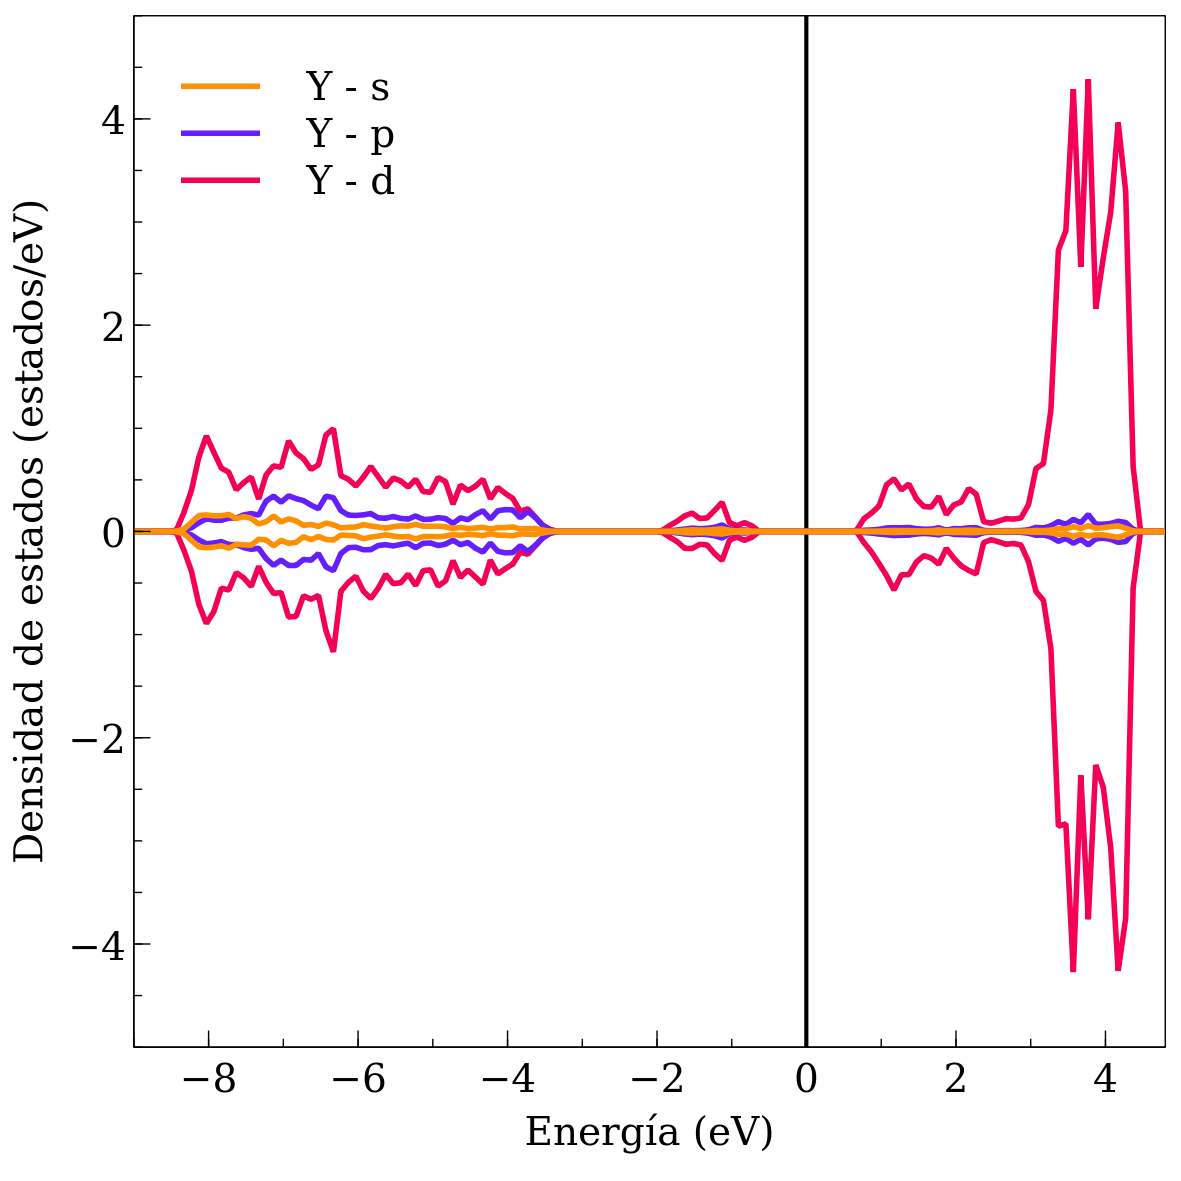
\includegraphics[width=0.5\textwidth]{contenido/resultados/cromita_itrio/img_cromita_itrio/YCrO3_DOS_Y_C_inf.png}}
    
    \subfloat[]{
        \label{yco_cr_c}
        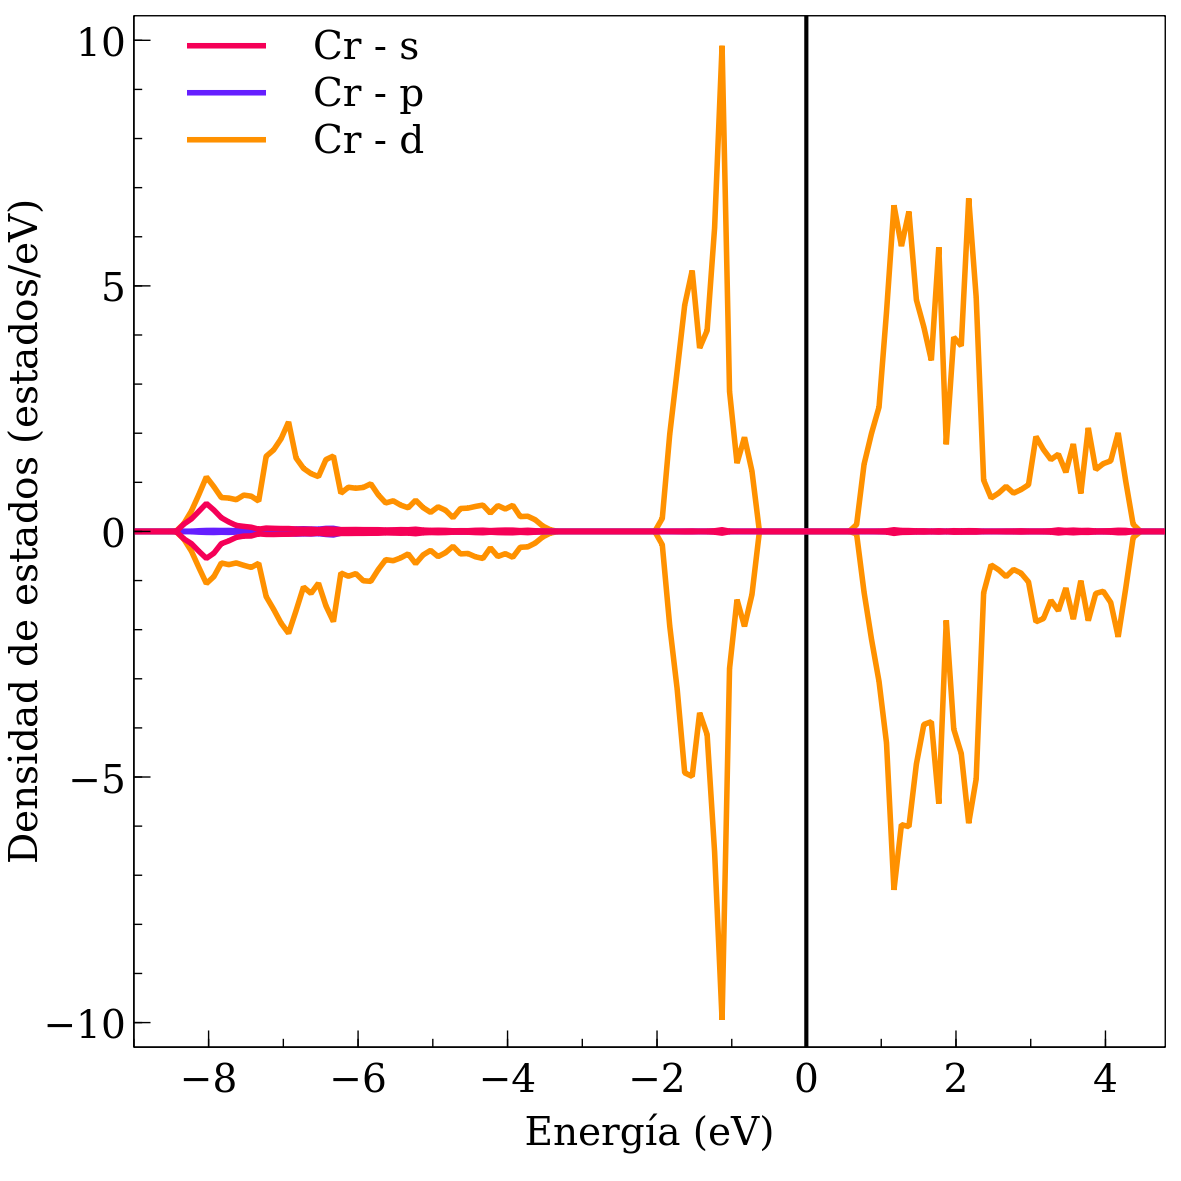
\includegraphics[width=0.5\textwidth]{contenido/resultados/cromita_itrio/img_cromita_itrio/YCrO3_DOS_Cr_C_inf.png}}
    \subfloat[]{
        \label{yco_o_c}
        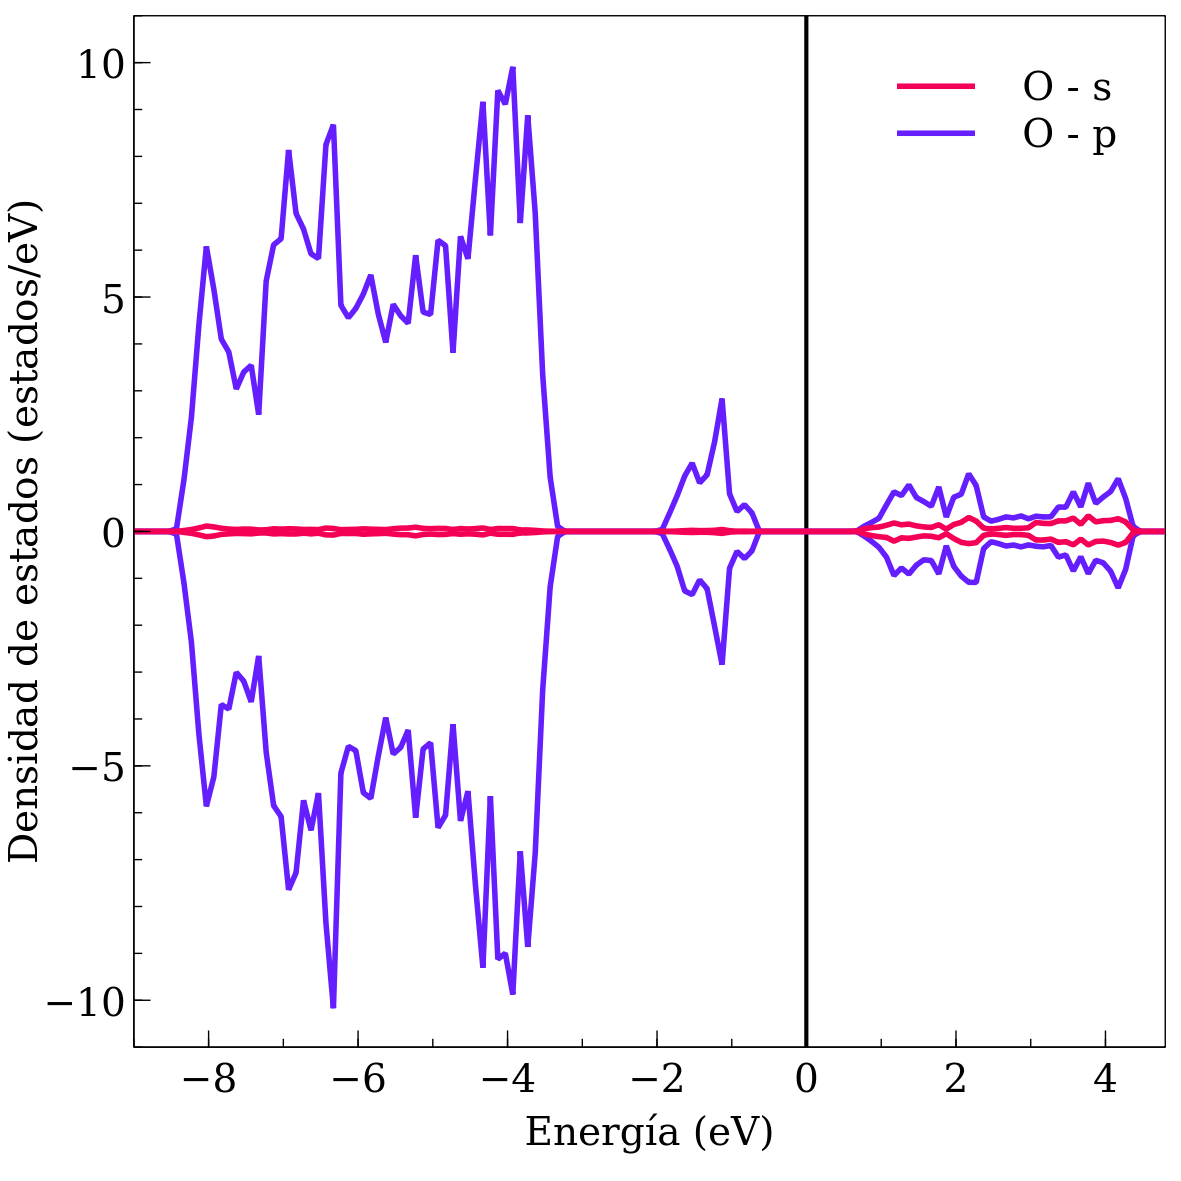
\includegraphics[width=0.5\textwidth]{contenido/resultados/cromita_itrio/img_cromita_itrio/YCrO3_DOS_O_C_inf.png}}
    \singlespace
    \caption[Densidad de estados del $YCrO_{3}$ con arreglo 
    antiferromagn\'etico 
    tipo C]{Densidad de estados del $YCrO_{3}$ con arreglo 
    antiferromagn\'etico 
        tipo C. La linea negra en cero indica el nivel de fermi. 
        \ref{yco_dos_c} \subref{yco_tot_c} 
        Densidad de 
        estados total y de cada elemento. \ref{yco_dos_c} \subref{yco_y_c} 
        Densidad de estados para 
        los orbitales s, 
        p, d del itrio. \ref{yco_dos_c} \subref{yco_cr_c} Densidad de estados 
        para los orbitales s, 
        p ,d del Cromo. 
        \ref{yco_dos_c} \subref{yco_o_c} Densidad de estados para los orbitales 
        s, p del Oxigeno.}
    \label{yco_dos_c}
\end{figure}


\noindent La figura \ref{yco_dos_c} \subref{yco_tot_c} muestra la densidad de 
estados total para 
cada 
elemento que compone el $YCrO_{3}$.Las energ\'ias fueron escaladas 
respecto al 
nivel de fermi que se tomo como cero de la escala horizontal, y la 
escala 
vertical positiva y negativa corresponden a los espines up y down 
respectivamente. En la banda de conducci\'on cerca del nivel de fermi 
hasta el nivel de energ\'ia 2 eV la densidad de estados de cromo es la 
mayor con un valor de 6 estados/eV seguida por las densidades de 
ox\'igeno e itrio que son peque\~nas por debajo de 2 estados/eV. A 
partir de 3 eV la densidad de estados de itrio es la mayor con 4 
estados/eV seguida por la densidad de estados de cromo y ox\'igeno que 
son similares con aproximadamente 2 estados/eV. En la banda de 
valencia cerca del nivel de fermi hasta -2 eV la densidad de estados 
de cromo es la dominante con un valor de 7 estados/eV seguida por una 
densidad m\'as peque\~na de estados de ox\'igeno y una densidad casi 
nula de estados de itrio. A partir de -4 eV hasta -8 eV la densidad de 
estados de ox\'igeno es la mayor con un valor cercano a 10 estados/eV, 
mezclados con estados de itrio y cromo cuyas densidades de estados son 
similares con un valor de aproximadamente 2 estados/eV


\noindent La figura \ref{yco_dos_c} \subref{yco_y_c} muestra la densidad de 
estados parcial del 
itrio para 
cada 
uno de los orbitales \textbf{s}, \textbf{p} y \textbf{d}.Las 
energ\'ias fueron escaladas 
respecto al 
nivel de fermi que se tomo como cero de la escala horizontal, y la 
escala 
vertical positiva y negativa corresponden a los espines up y down 
respectivamente. En la banda de conducci\'on cerca del nivel de fermi 
hasta 2 eV se puede observar una densidad peque\~na de orbitales 
\textbf{d}, a partir de este nivel de energ\'ia aumenta la densidad de 
orbitales \textbf{d} hasta 4 estados/eV. En todo el rango de energ\'ia 
de la banda de conducci\'on la contribuci\'on de los orbitales 
\textbf{s} y \textbf{p} no es apreciable. En la banda de valencia 
cerca del nivel de fermi aproximadamente en -2
 eV se observa una peque\~na densidad de orbitales \textbf{d} y la 
 densidad de los dem\'as orbitales en ese rango es nula. A partir de 
 -4 eV hasta -8 eV aumenta un poco la densidad de orbitales \textbf{d} 
 y la densidad de orbitales \textbf{p}; la contribuci\'on de los 
 orbitales \textbf{s} sigue siendo muy peque\~na en este rango de 
 energ\'ias.
 
 
 
 \noindent La figura \ref{yco_dos_c} \subref{yco_cr_c} muestra la densidad de 
 estados parcial del 
 cromo para 
 cada 
 uno de los orbitales \textbf{s}, \textbf{p} y \textbf{d}.Las 
 energ\'ias fueron escaladas 
 respecto al 
 nivel de fermi que se tomo como cero de la escala horizontal, y la 
 escala 
 vertical positiva y negativa corresponden a los espines up y down 
 respectivamente. En la banda de valencia se observa que la densidad 
 de los orbitales \textbf{d} es la predominante en todo el rango de 
 energ\'ias con un valor de 5 estados/eV y a partir del nivel de 
 energ\'ia de 3 eV la densidad desciende por debajo de 2 estados/eV. 
 La contribuci\'on de los orbitales \textbf{s} y \textbf{p} no es 
 apreciable. En la banda de valencia cerca del nivel de fermi hasta el 
 nivel de energ\'ia de -2 eV la densidad de orbitales  \textbf{d} es 
 la mayor con un valor cercano a 10 estados/eV. A partir de -4 eV 
 hasta -8 eV la densidad de orbitales \textbf{d} desciende por debajo 
 de 2 estados/eV. Al igual que en la banda de conducci\'on los 
 orbitales \textbf{s} y \textbf{p} no contribuyen de forma apreciable.
 
 
\noindent La figura \ref{yco_dos_c} \subref{yco_o_c} muestra la densidad de 
estados parcial del 
 ox''igeno para 
 cada 
 uno de los orbitales \textbf{s} y \textbf{p}. Las 
 energ\'ias fueron escaladas 
 respecto al 
 nivel de fermi que se tomo como cero de la escala horizontal, y la 
 escala 
 vertical positiva y negativa corresponden a los espines up y down 
 respectivamente. En la banda de conducci\'on la mayor densidad 
 pertenece a los orbitales \textbf{p} pero esta es reducida, dado que 
 tiene un valor por debajo de los 2 estados/eV y la contribuci\'on del 
 orbital \textbf{s} es casi nula. En la banda de valencia cerca al 
 nivel de fermi se observa un rango peque\~no de energ\'ias con una 
 densidad de orbitales \textbf{p} reducida de aproximadamente 2 
 estados/eV. A partir de -4 eV hasta -8 eV la densidad de orbitales 
 \textbf{p} es la mayor con un rango de valores desde 3 estados/eV 
 hasta 10 estados/eV. En este rango de energ\'ias la contribuci\'on de 
 los dem\'as orbitales es casi inexistente.
 
% ######################################################
% ######################################################

\subsection{Estructura de bandas de energ\'ia del $\mathbf{YCrO_{3}}$ con      
    arreglo antiferromagn\'etico tipo G}

% ----------------------------
% FIGURA: banda YCrO3 tipo G
% ----------------------------

\begin{figure}[H]
	\centering
	\includegraphics[width=0.7\textwidth]{contenido/resultados/cromita_itrio/img_cromita_itrio/YCrO3_bandas_G_inf.png}
	\singlespace
	\caption[Bandas de energ\'ia del $YCrO_{3}$ con arreglo 
	antiferromagn\'etico tipo G]{Estructura de bandas de energ\'ia del 
	$YCrO_{3}$ con arreglo antiferromagn\'etico tipo G. La l\'inea roja marca 
	el 
	nivel de fermi. Los puntos de alta simetr\'ia tomados en la primera zona de 
	brillouin son $\Gamma - X - S - Y - \Gamma$.}
	\label{yco_band_g}
\end{figure}


La figura \ref{yco_band_g} muestra la estructura de bandas de energ\'ia del 
$YCrO_{3}$ con arreglo antiferromagn\'etico tipo G.  Las energ\'ias 
fueron escaladas 
respecto al nivel de fermi, que es tomado como el cero de la escala 
vertical.Se observa un gap de 
energ\'ia de $1.6$ eV el cual es cercano al valor de $1.64$ reportado por otro 
estudio \cite{nair2013}. El gap esta definido entre el m\'inimo de la banda de 
conducci\'on ubicado en el punto $S$ 
y el m\'aximo de la banda de conducci\'on ubicado en el punto 
$\Gamma$. Por debajo 
del nivel de fermi en la banda de valencia 
alrededor del nivel de energ\'ia de -3 eV se observa una franja que no 
posee bandas de energ\'ia. Por sobre el nivel de fermi alrededor de 3 
eV se halla una regi\'on que no posee bandas de energ\'ia.


\subsection{Densidad de estados del $\mathbf{YCrO_{3}}$ con arreglo      
    antiferromagn\'etico tipo G}

% -------------------------------------------
% FIGURA: densidades de estado YCrO3 tipo G
% -------------------------------------------

\begin{figure}[H]
    \centering
    \subfloat[]{
        \label{yco_tot_g}
        \includegraphics[width=0.5\textwidth]{contenido/resultados/cromita_itrio/img_cromita_itrio/YCrO3_DOS_G_inf.png}}
    \subfloat[]{
        \label{yco_y_g}
        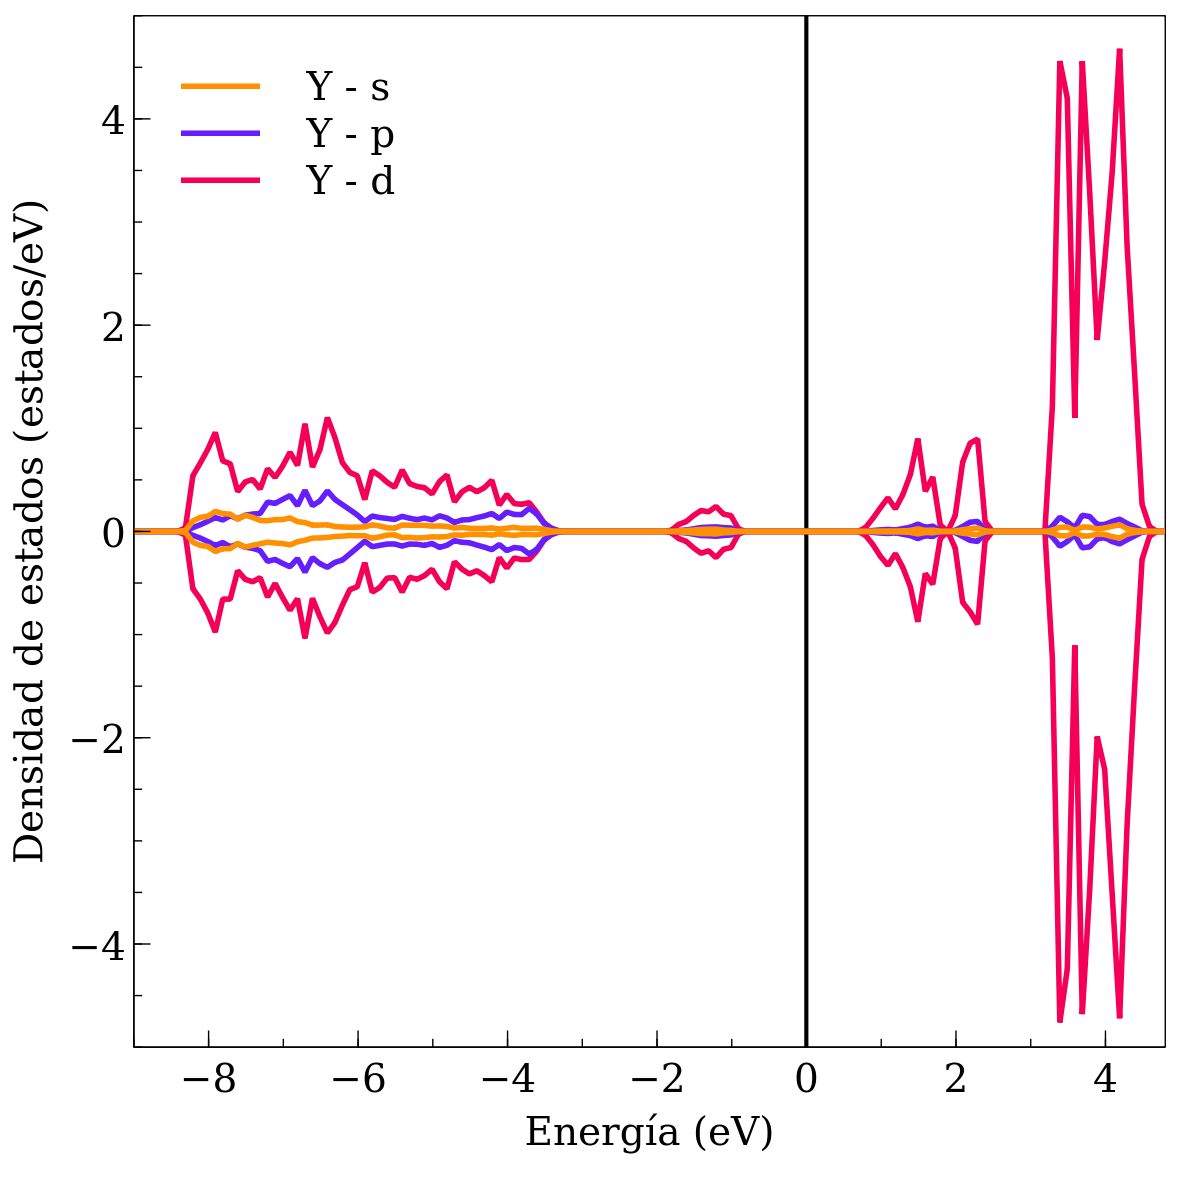
\includegraphics[width=0.5\textwidth]{contenido/resultados/cromita_itrio/img_cromita_itrio/YCrO3_DOS_Y_G_inf.png}}
    
    \subfloat[]{
        \label{yco_cr_g}
        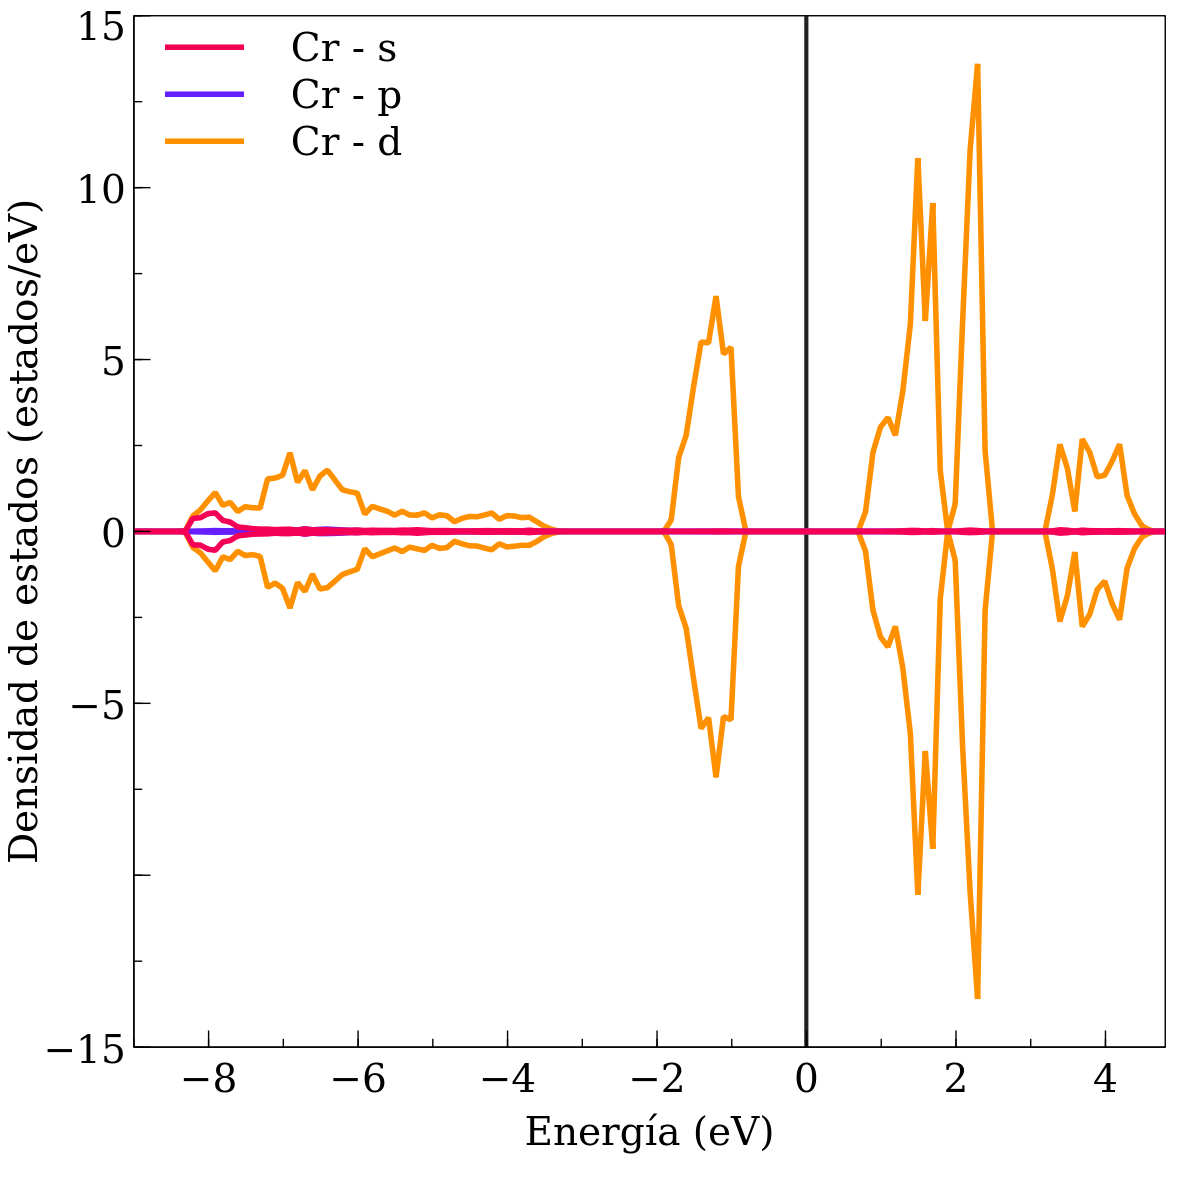
\includegraphics[width=0.5\textwidth]{contenido/resultados/cromita_itrio/img_cromita_itrio/YCrO3_DOS_Cr_G_inf.png}}
    \subfloat[]{
        \label{yco_o_g}
        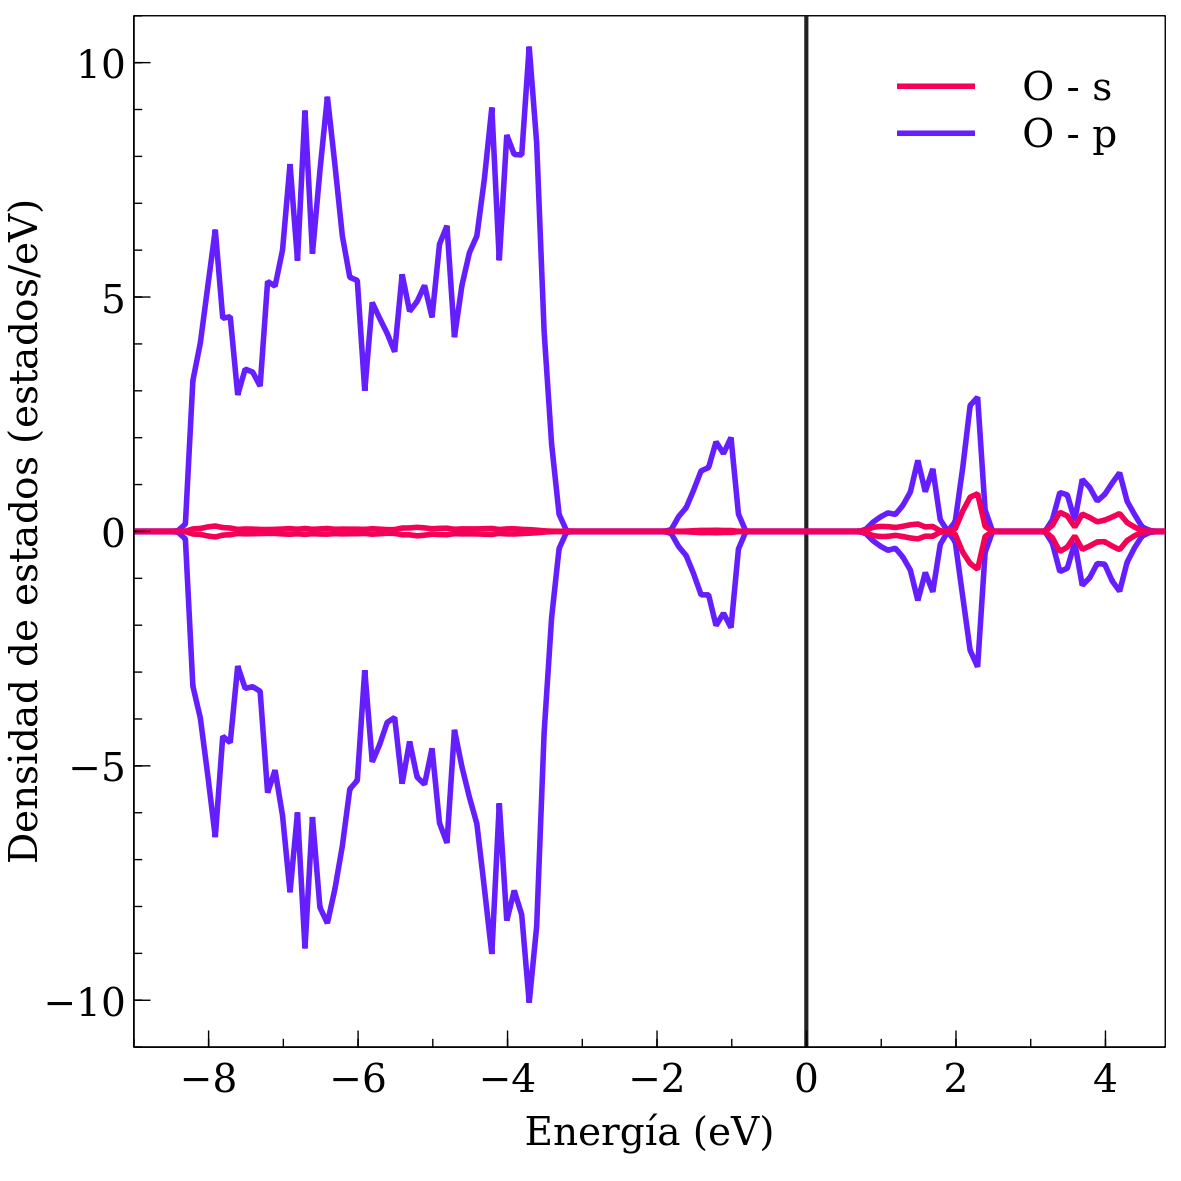
\includegraphics[width=0.5\textwidth]{contenido/resultados/cromita_itrio/img_cromita_itrio/YCrO3_DOS_O_G_inf.png}}
    \singlespace
    \caption[Densidad de estados del $YCrO_{3}$ con arreglo 
    antiferromagn\'etico 
    tipo G]{Densidad de estados del $YCrO_{3}$ con arreglo 
    antiferromagn\'etico 
        tipo G. La linea negra en cero indica el nivel de fermi. 
        \ref{yco_dos_g} \subref{yco_tot_g} 
        Densidad de 
        estados total y de cada elemento. \ref{yco_dos_g} \subref{yco_y_g} 
        Densidad de estados para 
        los orbitales s, 
        p, d del itrio. \ref{yco_dos_g} \subref{yco_cr_g} Densidad de estados 
        para los orbitales s, 
        p ,d del Cromo. 
        \ref{yco_dos_g} \subref{yco_o_g} Densidad de estados para los orbitales 
        s, p del Oxigeno.}
    \label{yco_dos_g}
\end{figure}


La figura \ref{yco_dos_g} \subref{yco_tot_g} muestra la densidad de estados 
total para 
cada 
elemento que compone el $YCrO_{3}$.Las energ\'ias fueron escaladas 
respecto al 
nivel de fermi que se tomo como cero de la escala horizontal, y la 
escala 
vertical positiva y negativa corresponden a los espines up y down 
respectivamente. En la banda de conducci\'on cerca del nivel de fermi 
hasta aproximadamente 2 eV se observa que la densidad de estados del 
cromo es la mayor con un m\'aximo de 10 estados/eV en ese rango de 
energ\'ias las densidades de estado del itrio y del ox\'igeno son 
reducidas con valores por debajo de 2 estados/eV. Alrededor de 3 eV se 
observa una zona que no esta ocupada por ning\'un estado. A partir de 
aproximadamente $3.5$ eV la mayor densidad pertenece al itrio con un 
valor de 4 estados/eV, tambi\'en se encuentran las densidades de cromo 
y ox\'igeno que son similares entre s\'i con un valor menor a 2 
estados/eV. En la banda de valencia cerca del nivel de fermi hasta 
aproximadamente -2 eV la mayor densidad pertenece al cromo con un 
valor de 6 estados/eV, tambi\'en se encuentran estados de ox\'igeno e 
itrio por debajo de los 2 estados/eV. En el rango de -4 eV hasta -8 eV 
el ox\'igeno posee la mayor densidad de estados con valores de entre 4 
estados/eV hasta 10 estados/eV, tambi\'en se encuentran estados de 
cromo e itrio cuyas densidades son similares con un valor por debajo 
de 3 estados/eV.


\noindent La figura \ref{yco_dos_g} \subref{yco_y_g} muestra la densidad de 
estados parcial del 
itrio para 
cada 
uno de los orbitales \textbf{s}, \textbf{p} y \textbf{d}.Las 
energ\'ias fueron escaladas 
respecto al 
nivel de fermi que se tomo como cero de la escala horizontal, y la 
escala 
vertical positiva y negativa corresponden a los espines up y down 
respectivamente. En la banda de conducci\'on cerca del nivel de fermi 
hasta aproximadamente $2.5$ eV se observa una peque\~na densidad de 
orbitales \textbf{d} con un valor de 1 estado/eV. Luego a partir de 3 
eV la densidad de orbitales \textbf{d} aumenta hasta 4 estados/eV. En 
todo el rango de energ\'ias de la banda de conducci\'on las 
contribuciones de los orbitales \textbf{s} y \textbf{p} no son 
apreciables. En la banda de valencia se observa una densidad de 
orbitales \textbf{d} peque\~na cerca del nivel de fermi. A partir de 
-4 eV hasta -8 eV la densidad de orbitales \textbf{d} es la mayor y  
se encuentra por debajo de 2 estados/eV, y en este rango los orbitales 
\textbf{s} y \textbf{p} tienen una densidad similar y bastante 
peque\~na.



\noindent La figura \ref{yco_dos_g} \subref{yco_cr_g} muestra la densidad de 
estados parcial del 
cromo para 
cada 
uno de los orbitales \textbf{s}, \textbf{p} y \textbf{d}.Las 
energ\'ias fueron escaladas 
respecto al 
nivel de fermi que se tomo como cero de la escala horizontal, y la 
escala 
vertical positiva y negativa corresponden a los espines up y down 
respectivamente. En la banda de conducci\'on se observa que los 
orbitales \textbf{d} tienen la mayor densidad en todo el rango de 
energ\'ias. Con valores de densidad de 10 estados/eV cerca del nivel 
de fermi hasta aproximadamente 2 eV. Luego la densidad se reduce por 
debajo de 3 estados/eV a partir del nivel de energ\'ia de 3 eV. Las 
contribuciones de los dem\'as orbitales son nulas en la banda de 
conducci\'on. En la banda de valencia cerca al nivel de fermi hasta -2 
eV se tiene una densidad de orbitales \textbf{d} con un valor 
aproximado de 6 estados/eV. Luego a partir de -4 eV hasta -8 eV la 
densidad se reduce por debajo de 3 estados/eV pero siguen predominando 
los orbitales \textbf{d}. En la banda de valencia tampoco existe una 
contribuci\'on apreciable de los orbitales \textbf{s} y \textbf{p}.


\noindent La figura \ref{yco_dos_g} \subref{yco_o_g} muestra la densidad de 
estados parcial del 
ox\'igeno para 
cada 
uno de los orbitales \textbf{s} y \textbf{p}.Las 
energ\'ias fueron escaladas 
respecto al 
nivel de fermi que se tomo como cero de la escala horizontal, y la 
escala 
vertical positiva y negativa corresponden a los espines up y down 
respectivamente. En la banda de conducci\'on cerca del nivel de fermi 
hasta aproximadamente 2 eV se observa una peque\~na densidad del 
orbital \textbf{p} con un valor por debajo de 3 estados/eV. Y 
alrededor de 4 eV tambi\'en se halla una densidad de los orbitales 
\textbf{p} peque\~na por debajo de 2 estados/eV. Adem\'as la 
contribuci\'on del orbital \textbf{s} en la banda de conducci\'on es 
reducida. En la banda de valencia cerca al nivel de fermi se observa 
una densidad peque\~na del orbital \textbf{p} por debajo de 2 
estados/eV. En el rango de -4 eV hasta -8 eV los orbitales \textbf{p} 
tienen la mayor densidad con valores entre 4 estados/eV hasta 10 
estados/eV. En la banda de valencia la contribuci\'on del orbital 
\textbf{s} no es significativa.

% ######################################################
% ######################################################

\subsection{Densidad de carga del $\mathbf{YCrO_{3}}$ con arreglos      
    antiferromagn\'eticos tipo A, C y G}

% ----------------------------
% FIGURA: densidades de carga
% ----------------------------

\begin{figure}[H]
	\centering
	\subfloat[]{
		\label{yco_DC_A}
		\includegraphics[width=0.33\textwidth]{contenido/resultados/cromita_itrio/img_cromita_itrio/YCrO3_DC_plano2_A.png}}
	\subfloat[]{
		\label{yco_DC_C}
		\includegraphics[width=0.33\textwidth]{contenido/resultados/cromita_itrio/img_cromita_itrio/YCrO3_DC_plano2_C.png}}
	\subfloat[]{
		\label{yco_DC_G}
		\includegraphics[width=0.33\textwidth]{contenido/resultados/cromita_itrio/img_cromita_itrio/YCrO3_DC_plano2_G.png}}
	\singlespace
	\caption[Densidades de carga del $YCrO_{3}$ con arreglos 
	antiferromagn\'eticos tipo A,C y G]{\ref{yco_DC} \subref{yco_DC_A} Densidad 
	de carga del arreglo 
	antiferromagn\'etico tipo A. \ref{yco_DC} \subref{yco_DC_C}  Densidad de 
	carga del arreglo 
	antiferromagn\'etico tipo C. \ref{yco_DC} \subref{yco_DC_G}  Densidad de 
	carga del arreglo 
	antiferromagn\'etico tipo G.}
	\label{yco_DC}
\end{figure}

La figura \ref{yco_DC} muestra la densidad de carga de los tres arreglos 
antiferromagn\'eticos, con el fin de poder estudiar el tipo de enlace que 
existe entre los \'atomos de cromo y ox\'igeno, debido a que se pudo observar 
en la gr\'afica de densidad de estados un mezcla entre los estados de estos 
\'atomos. La densidad de carga entre el cromo y el ox\'igeno es 
aproximadamente $0.3$ e/\AA$^{3}$ lo que indica que la interacci\'on no es 
solo i\'onica sino que puede considerarse covalente. De manera similar la 
interacci\'on entre el itrio y el ox\'igeno se asocia con una densidad de carga 
de $0.02$ e/\AA$^{3}$.

